\documentclass[10pt]{beamer}

\usepackage[T1]{fontenc}
\usepackage[french]{babel}
\usepackage{amsmath}
\usepackage{amssymb}
\usepackage{booktabs}
\usepackage{graphicx}
\usepackage{siunitx}
\usepackage{multirow}
\usepackage{libs/utils}
\usepackage{fancyvrb}
\usepackage[cache=false]{minted}
\setminted{fontsize=\tiny,frame=single}


% \usetheme{Madrid}

\usetheme{CambridgeUS}
\usecolortheme{spruce}

\setbeamertemplate{navigation symbols}{}
\setbeamertemplate{caption}[numbered]{}% Number float-like environments

% Make toc bullets dark green to match the theme
\setbeamercolor{section number projected}{bg=green!40!black,fg=white}
\setbeamercolor{subsection number projected}{bg=green!40!black,fg=white}
% Do the same for bullets in itemize/enumerate environments
\setbeamercolor{item projected}{bg=green!40!black,fg=white}
\setbeamercolor{subitem projected}{bg=green!40!black,fg=white}
\setbeamercolor{subsubitem projected}{bg=green!40!black,fg=white}
% Change the color of "Figure X -" in captions
\setbeamercolor{caption name}{fg=green!40!black}

\renewcommand{\frenchtablename}{Tableau}

\AtBeginSection[]{
	\begin{frame}[noframenumbering,plain]
  \vfill
  \centering
  \begin{beamercolorbox}[sep=8pt,center,shadow=true,rounded=true]{title}
    \usebeamerfont{title}\insertsectionhead\par%
  \end{beamercolorbox}
  \vfill
\end{frame}
}




% \usetheme{metropolis}

\title[Algèbre linéaire et filtres numériques]{S5-APP4: Algèbre linéaire et filtres numériques}
\author[Benjamin C. \& Shawn C.]{
  Benjamin Chausse (chab1704) \\
  Shawn Couture (cous1912)
}

\institute[UDS]{Université de Sherbrooke}
\date{\today}

\begin{document}
\maketitle

\begin{frame}
  \frametitle{Table des matières}
  \tableofcontents
\end{frame}

\section{Correction des aberrations}
\subsection{Filtre inverse et stabilité}

\begin{frame}
\frametitle{Filtre inverse et stabilité}
	\footnotesize{\begin{align}
		H(z) &= \frac{
				(z-0.9\e^{j\pi/2})
				(z-0.9\e^{-j\pi/2})
				(z-0.95\e^{j\pi/8})
				(z-0.95\e^{-j\pi/8})
		  }{
				z(z+0.99)^2(z-0.8)
			} \\ \nonumber \\
		H^{-1}(z)  &= \frac{
				z(z+0.99)^2(z-0.8)
		  }{
				(z-0.9\e^{j\pi/2})
				(z-0.9\e^{-j\pi/2})
				(z-0.95\e^{j\pi/8})
				(z-0.95\e^{-j\pi/8})
			}
	\end{align}}
	% \begin{columns}[t] % Align columns at the top
	\begin{columns}
		\begin{column}{0.5\textwidth}
			\begin{table}
				\caption{Identités du filtre aberrant}
				\begin{tabular}{lll}
					\toprule
					Identité & Dans $H(Z)$ & Dans $H^{-1}(z)$ \\
					\midrule
					$0$                & $|\textrm{pôle}| <0$ & zéro \\
					$0.8$              & $|\textrm{pôle}| <0$ & zéro \\
					$-0.99$            & $|\textrm{pôle}| <0$ & zéro \\
					$0.9\e^{j\pi/2}$   & zéro & $|\textrm{pôle}| <0$ \\
					$0.9\e^{-j\pi/2}$  & zéro & $|\textrm{pôle}| <0$ \\
					$0.95\e^{j\pi/8}$  & zéro & $|\textrm{pôle}| <0$ \\
					$0.95\e^{-j\pi/8}$ & zéro & $|\textrm{pôle}| <0$ \\
					\bottomrule
				\end{tabular}
			\end{table}
		\end{column}
		\begin{column}{0.5\textwidth}
			\textbf{Réponse dans $\mathbb{R}$}: \\
			(pôles/zéros complexes ont leur conjugé) \\
			\begin{itemize}
				\item $0$ purement réel
				\item $0.8$ purement réel
				\item $-0.99$ purement réel\footnotemark[1]
				\item $0.9\e^{j\pi/2}\leftrightharpoons0.9\e^{-j\pi/2}$
				\item $0.95\e^{j\pi/8}\leftrightharpoons0.95\e^{-j\pi/8}$
			\end{itemize}
		\end{column}
	\end{columns}
		\footnotetext[1]{Puisque qu'il est élevé au carré, ce zéro est présent deux
		fois dans le filtre}
\end{frame}

\begin{frame}
\frametitle{Résultats}

	\begin{columns}[t]
		\begin{column}{0.32\textwidth}
			\begin{figure}
				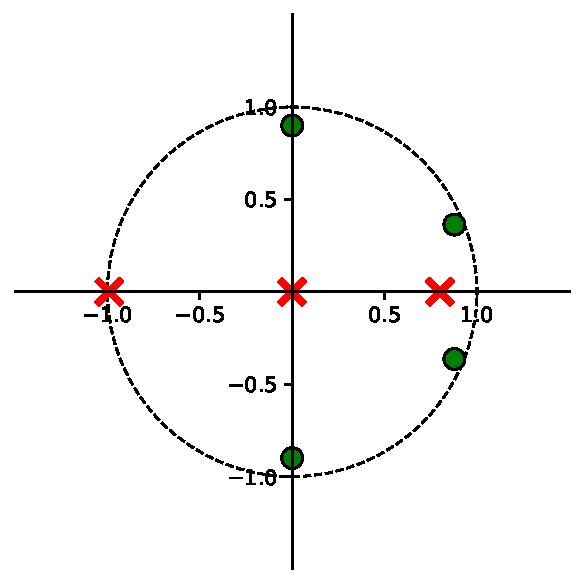
\includegraphics[width=1\linewidth]{figures/aberration-zplane-inv.pdf}
				\caption{\footnotesize{Filtre réparateur}}
			\end{figure}
		\end{column}

		\begin{column}{0.32\textwidth}
			\begin{figure}
				
\includegraphics[width=\linewidth]{figures/aberration-before.png}
				\caption{\footnotesize{Avec l'aberration}}
			\end{figure}
		\end{column}

		\begin{column}{0.32\textwidth}
			\begin{figure}
				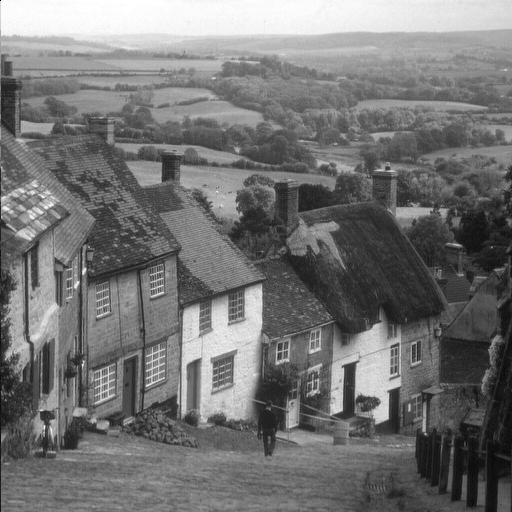
\includegraphics[width=\linewidth]{figures/aberration-after.png}
				\caption{\footnotesize{Aberration corrigée}}
			\end{figure}
		\end{column}
	\end{columns}

\end{frame}


\section{Rotation de l'image}
\renewcommand{\e}{\vec{e_1}}
\newcommand{\ee}{\vec{e_2}}

\renewcommand{\u}{\vec{u_1}}
\newcommand{\uu}{\vec{u_2}}

\renewcommand{\v}{v_1}
\newcommand{\vv}{v_2}

\newcommand{\vp}{v_1^\prime}
\newcommand{\vvp}{v_2^\prime}
\newcommand{\hpi}{\frac{-\pi}{2}}


\begin{frame}
	\begin{columns}[t]
		\begin{column}{0.6\textwidth}
			\textbf{Changement de base:}
			\quickfigure{\footnotesize{Changement de base}}{base-change
			}{.66}{base-change.png}\vspace{-.7cm}

			\footnotesize{\begin{align}
					E &= \{ \e, \ee \}
					&U = \{ \u, \uu \} \\
					\e &= 0\u + (-1)\uu
					&\ee = \u + 0\uu
			\end{align}
			\begin{align}
					\v\e + \vv\ee &= \vp\u + \vvp\uu \\
					\v(0\u - \uu) + \vv(\u + 0\uu) &= \vp\u + \vvp\uu \\
					(0\v + \vv)\u + (-\v + 0\vv)\uu &= \vp\u + \vvp\uu \\
					\begin{bmatrix} 0 & 1 \\ -1 & 0 \end{bmatrix}
					\begin{bmatrix} \v \\ \vv \end{bmatrix} &=
					\begin{bmatrix} \vp \\ \vvp \end{bmatrix}
			\end{align}}


		\end{column}
		\begin{column}{0.4\textwidth}
		\textbf{Matrice de passage:}

		\footnotesize{\begin{align}
		\theta &= \hpi \\
		T &= \begin{bmatrix}
						\cos\theta & -\sin\theta \\
						\sin\theta & \cos\theta \\
         \end{bmatrix} \\
		T &= \begin{bmatrix}
						\cos\hpi & -\sin\hpi \\
						\sin\hpi & \cos\hpi \\
         \end{bmatrix} \\
		T &= \begin{bmatrix}
						0 & 1 \\
						-1 & 0 \\
         \end{bmatrix}
		\end{align}}

		\quickfigure{
			\tiny{Exemple de rotation}
		}{rotated-example}{.6}{rotated-example.png}

		\end{column}
	\end{columns}
\end{frame}

\begin{frame}[fragile]
\thead{Implémentation \textit{Python}}
\begin{minted}{python}
def get_transformation_array(angle: float):
    radians = np.deg2rad(angle)
    sin = np.round(np.sin(radians), decimals=10)
    cos = np.round(np.cos(radians), decimals=10)
    return np.array([[cos, -sin], [sin, cos]])

def rotate_picture(image: np.ndarray, angle: float):
    R = get_transformation_array(angle)
    h, w = image.shape
    rotated = np.zeros((h, w))
    center_x = (w - 1) / 2
    center_y = (h - 1) / 2
    x = np.arange(w)            # Output grid (destination pixels)
    y = np.arange(h)
    xx, yy = np.meshgrid(x, y)
    x_shifted = xx - center_x	# Shift origin to center
    y_shifted = yy - center_y
    coords = np.vstack((x_shifted.ravel(), y_shifted.ravel()))
    source_coords = R.T @ coords # Map BACK into source image
    ip = (source_coords[0] + center_x).round().astype(int)
    jp = (source_coords[1] + center_y).round().astype(int)
    ip = ip.reshape(h, w)
    jp = jp.reshape(h, w)
    mask = (0 <= ip) & (ip < w) & (0 <= jp) & (jp < h)
    rotated[mask] = image[jp[mask], ip[mask]]
    return rotated
\end{minted}
\end{frame}


\section{Débruitage}
\subsection{Transformation bilinéaire - (Approche mathématique)}

% Tu peux changer les noms de diapos si tu veux.
% Je trouvais ca logique d'avoir theorie+resultats mais tu vas peut-etre vouloir
% autre chose

\begin{frame}
\frametitle{Transformation bilinéaire — Théorie}
\begin{enumerate}
    \item Normalization des fréquences digitals
    \item Application de la distortion (gauchissement des fréquences)
	\item Remplacement dans l'équation donnée
	\item Conversion de $s$ en $z$
	\item Simplifications
\end{enumerate}
\end{frame}

\begin{frame}
	\frametitle{Transformation bilinéaire}
	\begin{columns}[t]
		\begin{column}{0.4\textwidth}
			\textbf{Conversion en fréquences}:
			\footnotesize{\begin{align}
				f_e &= 1600 \nonumber \\
				f_c &= 500\,\text{Hz} \nonumber \\
		    \bar{\omega}_d&=\frac{2\pi f_d}{f_e} \\
				\bar\omega_c&=\frac{5\pi}{8} \\
				\omega_a&=\frac{2}{T_e}\tan\left(\frac{\bar\omega_d}{2}\right) \\
				\omega_c&=4789.14 \nonumber
			\end{align}}

		\end{column}
		\begin{column}{0.6\textwidth}
			\textbf{Remplacement dans l'équation donnée}:
			\footnotesize{\begin{align}
				H(s)&=\frac{1}{(\frac{s}{\omega_c})^2+\sqrt2(\frac{s}{\omega_c})+1} \\
				H(s)&=\frac{1}{(\frac{s}{4789.14})^2+\sqrt2(\frac{s}{4789.14})+1} \\
				s&=\frac{2}{T_e}\cdot\frac{1-z^{-1}}{1+z^{-1}} \\
				H(z)&=\frac{1}{
				(\frac{
				3200\frac{1-z^{-1}}{1+z^{-1}}}
				{4789.14})^2
				+\sqrt2
				(\frac{
				3200\frac{1-z^{-1}}{1+z^{-1}}
				}{4789.14})
				+1}
			\end{align}}

		\end{column}
	\end{columns}
\end{frame}

\begin{frame}
\frametitle{Transformation bilinéaire — Résultats}
\textbf{Équation obtenue:}
	\begin{equation}
		H(z) = \frac{ z^2 + 2z + 1 }{ 2.39z^2 + 1.1z + 0.505 }
	\end{equation}

	\begin{columns}

		\begin{column}{0.5\textwidth}
			\quickfigure{\footnotesize{Filtre manuel en fréquences}}{denoise-hand-freq
			}{}{denoise-hand-freq.pdf}
		\end{column}

		\begin{column}{0.5\textwidth}
			\quickfigure{\footnotesize{Filtre manuel $z$}}{denoise-zplane-hand
			}{.5}{denoise-zplane-hand.pdf}
		\end{column}

	\end{columns}
\end{frame}


\subsection{Approche Python}

\begin{frame}
\frametitle{Approche Python — Conception}
	\begin{columns}
		\begin{column}{0.5\textwidth}

			\quickfigure{
				\footnotesize{Filtre Butterworth}
			}{noise-test-butter}{}{denoise-butterworth.pdf}

			\quickfigure{
				\footnotesize{Filtre Élliptique (choisi)}
			}{noise-test-butter}{}{denoise-elliptic.pdf}

		\end{column}
		\begin{column}{0.5\textwidth}

			\quickfigure{
				\footnotesize{Filtre Chebyshev Type I}
			}{noise-test-butter}{}{denoise-chebyshev-i.pdf}

			\quickfigure{
				\footnotesize{Filtre Chebyshev Type II}
			}{noise-test-butter}{}{denoise-chebyshev-ii.pdf}

		\end{column}
	\end{columns}
\end{frame}

\begin{frame}
\frametitle{Approche Python — Choix final: Elliptique d'ordre 3}

			\quickfigure{
				\footnotesize{Filtre \textit{Python} choisi en $z$}
			}{noise-zplane-final}{.45}{denoise-zplane-final.pdf}

\end{frame}

\subsection{Comparaison des méthodes}

\begin{frame}
\frametitle{Comparaison des méthodes}
	\begin{columns}

		\begin{column}{0.32\textwidth}
			\quickfigure{\footnotesize{Image bruitée}}{denoise-result-orig
			}{}{denoise-result-orig.png}
		\end{column}

		\begin{column}{0.32\textwidth}
			\quickfigure{\footnotesize{Filtre manuel}}{denoise-result-hand
			}{}{denoise-result-hand.png}
		\end{column}

		\begin{column}{0.32\textwidth}
			\quickfigure{\footnotesize{Filtre \textit{Python}}}{denoise-result-python
			}{}{denoise-result-python.png}
		\end{column}

	\end{columns}
\end{frame}



\section{Compression d'image}

\begin{frame}
    \frametitle{Compression Matrice A — Théorie}
    \begin{enumerate}
        \item Obtenir la matrice de covariance
        \begin{enumerate}
            \item Analyze des données (colonnes)
            \item Construction du vecteur moyen
            \item Centrage des données
            \item Transposé de la matrice
            \item Produit matricielle
        \end{enumerate}
        \item Valeurs propres
        \begin{enumerate}
            \item Application de la formule
            \item Déterminant de la matrice
            \item Valeurs $\lambda$ qui donnent $0$
        \end{enumerate}
        \item Vecteurs propres
        \begin{enumerate}
            \item $\Sigma-\lambda I$ pour chaque $\lambda$ trouvé sachant $\Sigma v=\lambda v$
            \item Isolé $x$ et $y$ de chaque lignes (confirmation)
            \item Posé une valeur ($x$ ou $y$)
            \item Résolution pour trouvé la manquante
        \end{enumerate}
    \end{enumerate}
\end{frame}


\begin{frame}
    \frametitle{Déterminants et valeurs propres}
		\begin{columns}[t]

		\begin{column}{.5\linewidth}
		\textbf{Déterminant}:
			\footnotesize{\begin{align}
			\det(A-\lambda I)&=0 \\
        \det\left(
        \begin{bmatrix}
            4-\lambda&1\\
            2&5-\lambda
        \end{bmatrix}
        \right)&=0 \\
        \det\left(
            \begin{bmatrix}
                a&b\\
                c&d
            \end{bmatrix}
        \right)
				&=
        ad-bc \\
				(4-\lambda)(5-\lambda)-(1)(2) &= \det\\
				-\lambda^2-9\lambda+18 &= \det
			\end{align}}

		\end{column}
		\begin{column}{.5\linewidth}
		\textbf{Valeurs propres}:
			\footnotesize{
				\begin{align}
				\lambda   &= \frac{-b\pm\sqrt{b^2-4ac}}{2a} \\
				\lambda   &= \frac{9\pm3}{2}
				\end{align}
				\begin{align}
				\lambda_1 &= \frac{9-3}{2} & \lambda_2 &= \frac{9+3}{2} \\
				\lambda_1 &= 3             & \lambda_2 &= 6
			\end{align}}

		\end{column}
	\end{columns}
\end{frame}


\begin{frame}
    \frametitle{Matrice A - Vecteurs propres - Fonctions}

		\begin{columns}
		\begin{column}{0.5\textwidth}

			\scriptsize{\begin{align}
			A&-\lambda I \nonumber \\
				\lambda_2&=6 \nonumber \\
				\begin{bmatrix} 4&1\\ 2&5 \end{bmatrix}
				  - \begin{bmatrix} 6&0\\ 0&6 \end{bmatrix}
				  &= \begin{bmatrix} -2&1\\ 2&-1 \end{bmatrix} \\
				\begin{bmatrix} -2&1\\ 2&-1 \end{bmatrix}
				  \begin{bmatrix} x\\y \end{bmatrix}
				  &= \begin{bmatrix} 0\\0 \end{bmatrix} \\
				-2x+1y&=0 \\
				2x-1y&=0 \\
				2x-y&=0
			\end{align}}
		\end{column}

		\begin{column}{0.5\textwidth}
			\scriptsize{\begin{align}
				A \vec v&=\lambda\vec v \nonumber\\
				\lambda_1&=3 \nonumber\\
				\begin{bmatrix} 4&1\\ 2&5 \end{bmatrix}
					- \begin{bmatrix} 3&0\\ 0&3 \end{bmatrix}
					&= \begin{bmatrix} 1&1\\ 2&2 \end{bmatrix} \\
				\begin{bmatrix} 1&1\\ 2&2 \end{bmatrix}
					\begin{bmatrix} x\\y \end{bmatrix}
					&= \begin{bmatrix} 0\\0 \end{bmatrix} \\
				1x+1y&=0 \\
				2x+2y&=0 \\
				x-y&=0
			\end{align}}
		\end{column}
	\end{columns}

	\begin{columns}
		\begin{column}{0.3\textwidth}
			\quickfigure{
				\scriptsize{Original}
			}{compressed-original}{.7}{compressed-original.png}
		\end{column}
		\begin{column}{0.3\textwidth}
			\quickfigure{
				\scriptsize{Compression 50\%}
			}{compressed-fifty}{.7}{compressed-fifty.png}
		\end{column}
		\begin{column}{0.3\textwidth}
			\quickfigure{
				\scriptsize{Compression 70\%}
			}{compressed-seventy}{.7}{compressed-seventy.png}
		\end{column}

	\end{columns}

\end{frame}

\begin{frame}[fragile]
\begin{minted}{python}
def compute_change_of_basis(image: np.ndarray, change_of_basis_matrix: np.ndarray):
    return image @ change_of_basis_matrix.T
\end{minted}

\begin{columns}[t]
\begin{column}{0.5\linewidth}
\begin{minted}{python}
cov, mean, centered = get_covariance_matrix(image)
eigenvalues, eigenvectors = get_eigen(cov)
P = get_change_of_basis_matrix(eigenvectors)
projected = compute_change_of_basis(centered, P)
compressed = compress_projected(projected, keep_ratio)
reconstructed = reconstruct_image(compressed, P, mean)
\end{minted}

\begin{minted}{python}
def get_covariance_matrix(image: np.ndarray):
    mean = np.mean(image, axis=0)
    centered = image - mean
    covariance = np.cov(centered, rowvar=False)
    return covariance, mean, centered
\end{minted}

\begin{minted}{python}
def get_eigen(covariance: np.ndarray):
    eigenvalues, eigenvectors = np.linalg.eig(covariance)
    idx = np.argsort(eigenvalues)[::-1] # Tri décroissant
    return eigenvalues[idx], eigenvectors[:, idx]
\end{minted}
\end{column}
\begin{column}{0.5\linewidth}
\begin{minted}{python}
def get_change_of_basis_matrix(eigenvectors: np.ndarray):
    return eigenvectors.T
\end{minted}

\begin{minted}{python}
def reconstruct_image(compressed, change_of_basis_matrix, mean):
    reconstructed = compressed @ change_of_basis_matrix
    return reconstructed += mean
\end{minted}

\begin{minted}{python}
def compress_projected(projected: np.ndarray, keep_ratio: float):
    compressed = projected.copy()
    n_components = projected.shape[1]
    k = int(n_components * keep_ratio)
    compressed[:, k:] = 0
    return compressed
\end{minted}
\end{column}
\end{columns}
\end{frame}


\section{Conclusion}

\newcommand{\portion}{0.2}

\begin{frame}[fragile]
\frametitle{Conclusion}
	\begin{columns}[t]

	\begin{column}{\portion\linewidth}
		\quickfigure{
			\tiny{Originelle}
		}{complete-initial}{}{complete-initial.png}
	\end{column}

	\begin{column}{\portion\linewidth}
		\quickfigure{
			\tiny{Sans aberrations}
		}{complete-no-aberration}{}{complete-no-aberration.png}
	\end{column}

	\begin{column}{\portion\linewidth}
		\quickfigure{
			\tiny{Tournée}
		}{complete-rotated}{}{complete-rotated.png}
	\end{column}

	\begin{column}{\portion\linewidth}
		\quickfigure{
			\tiny{Débruitée}
		}{complete-denoised}{}{complete-denoised.png}
	\end{column}

	\begin{column}{\portion\linewidth}
		\quickfigure{
			\tiny{Compressée}
		}{complete-compressed}{}{complete-compressed.png}
	\end{column}

\end{columns}
\end{frame}

% \footnotesize{\begin{Verbatim}[frame=single]
% def load_png(path: str) -> np.ndarray:
%     plt.gray()
%     data = mpimg.imread(path)
%     if data.ndim == 3:
%         return np.mean(data, -1)
%     return data
% \end{Verbatim}}
% \tiny{\begin{Verbatim}[frame=single]
% def load_png(path: str) -> np.ndarray:
%     plt.gray()
%     data = mpimg.imread(path)
%     if data.ndim == 3:
%         return np.mean(data, -1)
%     return data
% \end{Verbatim}}



% \begin{frame}
% \frametitle{Merci}
% 	\begin{figure}
% 		\includegraphics[width=.9\linewidth]{figures/toulouse.jpg}
% 	\end{figure}
% \end{frame}


\end{document}
